\documentclass[a4paper,12pt,twoside]{book}
\usepackage[banglamainfont=Kalpurush, banglattfont=Siyam Rupali]{latexbangla}
\usepackage{hyperref}
\hypersetup{
	colorlinks=true,
	linkcolor=black,
	filecolor=magenta,      
	urlcolor=cyan,
}
\usepackage{fancyhdr}
\pagestyle{fancy}
\fancyhf{}
\fancyhead[RE,LO]{\leftmark}
\fancyhead[LE,RO]{\thepage}

\usepackage{amsmath}
\usepackage{amsthm}
\usepackage{units}
\usepackage{tikz}
\usetikzlibrary{matrix,arrows,decorations.pathmorphing}
\usepackage{blkarray}
\usepackage{color}
\usepackage{tcolorbox}
\usepackage{wrapfig}

\newtheorem{corollary}{অনুসিদ্ধান্ত}[section]
\setcounter{chapter}{1}
\begin{document}
	\chapter{ভেক্টর}
	{\Large Vector}\\
	\rule{\textwidth}{2pt}
	\newpage
\section*{রাশি ও সদিক রেখাংশ}
\begin{tcolorbox}[colback=green!5!white, colframe=green!75!black, title=রাশি]
	ভৌত জগতে যা কিছু পরিমাপ করা যায়, তাকে রাশি বলে।
	রাশি ২ প্রকারের। যথাঃ
	\begin{enumerate}
		\item অদিক রাশি বা স্কেলার রাশি (Scalar):\\
		সম্পূর্ণরূপে প্রকাশ করতে শুধু মান প্রয়োজন। যেমনঃ দৈর্ঘ্য, দূরত্ব, ভর, আয়তন ইত্যাদি।
		\item সদিক রাশি বা ভেক্টর রাশি (Vector):\\
		সম্পূর্ণরূপে প্রকাশ করতে মান এবং দিক উভয়ই প্রয়োজন। যেমনঃ বল, সরণ, বেগ, ত্বরণ ইত্যাদি। 
	\end{enumerate}
\end{tcolorbox}
\begin{figure}[h]
	\centering
	

\tikzset{every picture/.style={line width=0.75pt}} %set default line width to 0.75pt        

\begin{tikzpicture}[x=0.75pt,y=0.75pt,yscale=-0.8,xscale=0.8]
%uncomment if require: \path (0,300); %set diagram left start at 0, and has height of 300

%Straight Lines [id:da1353668082852677] 
\draw    (224,170) -- (403.78,86.27) ;
\draw [shift={(406.5,85)}, rotate = 515.03] [fill={rgb, 255:red, 0; green, 0; blue, 0 }  ][line width=0.08]  [draw opacity=0] (10.72,-5.15) -- (0,0) -- (10.72,5.15) -- (7.12,0) -- cycle    ;
\draw [shift={(224,170)}, rotate = 335.03] [color={rgb, 255:red, 0; green, 0; blue, 0 }  ][fill={rgb, 255:red, 0; green, 0; blue, 0 }  ][line width=0.75]      (0, 0) circle [x radius= 3.35, y radius= 3.35]   ;
%Curve Lines [id:da7159902870257879] 
\draw    (149.5,146) .. controls (154.48,137.04) and (174.3,95.42) .. (208.98,159.03) ;
\draw [shift={(209.5,160)}, rotate = 241.7] [color={rgb, 255:red, 0; green, 0; blue, 0 }  ][line width=0.75]    (10.93,-3.29) .. controls (6.95,-1.4) and (3.31,-0.3) .. (0,0) .. controls (3.31,0.3) and (6.95,1.4) .. (10.93,3.29)   ;
%Curve Lines [id:da3699293995971742] 
\draw    (462.5,63) .. controls (431.97,31.48) and (414.04,42.65) .. (403.96,75.48) ;
\draw [shift={(403.5,77)}, rotate = 286.39] [color={rgb, 255:red, 0; green, 0; blue, 0 }  ][line width=0.75]    (10.93,-3.29) .. controls (6.95,-1.4) and (3.31,-0.3) .. (0,0) .. controls (3.31,0.3) and (6.95,1.4) .. (10.93,3.29)   ;

% Text Node
\draw (98,152) node [anchor=north west][inner sep=0.75pt]   [align=left] {Initial Point};
% Text Node
\draw (455,68) node [anchor=north west][inner sep=0.75pt]   [align=left] {Terminal Point};
% Text Node
\draw (201,167.4) node [anchor=north west][inner sep=0.75pt]    {$A$};
% Text Node
\draw (409,76.4) node [anchor=north west][inner sep=0.75pt]    {$B$};


\end{tikzpicture}
	\caption{সদিক রেখাংশ (Directed Line Segment)}
	\label{vec-fig}
\end{figure}
\begin{tcolorbox}[colback=green!5!white, colframe=green!75!black,title=দিক নির্দেশক রেখাংশ বা সদিক রেখাংশ] 
	কোনো সরলরেখার এক প্রান্তকে আদিবিন্দু (Initial Point) এবং অপর প্রান্তকে অন্তবিন্দু (Terminal Point) হিসেবে চিহ্নিত করলেই, ঐ সরলরেখাটি একটি দিক নির্দেশক রেখাংশ বা সদিক রেখাংশ (directed line segment) হবে। কোনো সরলরেখার আদিবিন্দু $A$ এবং অন্তবিন্দু $B$ হলে, $AB$ রেখাংশটি একটি সদিক রেখাংশ যাকে $\overrightarrow{AB}$ দ্বারা প্রকাশ করা হয়। $\overrightarrow{AB}$ এর দিক হবে $A$ (initial point) থেকে $B$ (terminal point) এর দিকে।
\end{tcolorbox}
\newpage
\section*{ভেক্টরের ধারক ও সমতা }
\begin{figure}[h]
	\centering
	
\tikzset{every picture/.style={line width=0.75pt}} %set default line width to 0.75pt        

\begin{tikzpicture}[x=0.75pt,y=0.75pt,yscale=-1,xscale=1]
%uncomment if require: \path (0,300); %set diagram left start at 0, and has height of 300

%Straight Lines [id:da319143912657855] 
\draw    (175,179) -- (455.5,95) ;
%Straight Lines [id:da7931344610645972] 
\draw [color={rgb, 255:red, 74; green, 144; blue, 226 }  ,draw opacity=1]  (259.75,154) -- (367.88,120.88) ;
\draw [shift={(370.75,120)}, rotate = 522.97] [fill={rgb, 255:red, 74; green, 144; blue, 226 }  ,fill opacity=1 ][line width=0.08]  [draw opacity=0] (10.72,-5.15) -- (0,0) -- (10.72,5.15) -- (7.12,0) -- cycle    ;
\draw [shift={(259.75,154)}, rotate = 342.97] [color={rgb, 255:red, 74; green, 144; blue, 226 }  ,draw opacity=1 ][fill={rgb, 255:red, 74; green, 144; blue, 226 }  ,fill opacity=1 ][line width=0.75]      (0, 0) circle [x radius= 3.35, y radius= 3.35]   ;

% Text Node
\draw (155,177.4) node [anchor=north west][inner sep=0.75pt]    {$X$};
% Text Node
\draw (462,82.4) node [anchor=north west][inner sep=0.75pt]    {$Y$};
% Text Node
\draw (248,127.4) node [anchor=north west][inner sep=0.75pt]  [color={rgb, 255:red, 74; green, 144; blue, 226 }  ,opacity=1 ]  {$A$};
% Text Node
\draw (365,96.4) node [anchor=north west][inner sep=0.75pt]  [color={rgb, 255:red, 74; green, 144; blue, 226 }  ,opacity=1 ]  {$B$};

\draw (300,105.4) node [anchor=north west] [color={rgb, 255:red, 74; green, 144; blue, 226 }  ,opacity=1 ] {$\underline{a}$};


\end{tikzpicture}
	\caption{ভেক্টর এর ধারক}
	\label{vec-fig-1}
\end{figure}
\begin{itemize}
	\item[$(i)$] \textbf{ধারক (Support):} কোনো ভেক্টর নির্দেশক সদিক রেখাংশ যে অসীম সরলরেখার অংশ, তাকে ঐ ভেক্টরের ধারক রেখা বলে। চিত্র \ref{vec-fig-1} এ $\overrightarrow{AB}$ বা $\underline{a}$ এর ধারক $XY$। 
	\item[$(ii)$] \textbf{মান (Magnitude):} ভেক্টরের আদিবিন্দু ও অন্তবিন্দুর মধ্যবর্তী দূরত্বকে ঐ ভেক্টরের মান বলে। $\overrightarrow{AB}$ বা $\underline{a}$ ভেক্টর এর মানকে $|\overrightarrow{AB}|=a$ দ্বারা প্রকাশ করা হয়। 
	\item[$(iii)$] \textbf{দিক (Sense or Direction):} ভেক্টরের দিক হবে আদিবিন্দু হতে অন্তবিন্দুর দিকে। $\overrightarrow{AB}$ এর দিক $A$ বিন্দু থেকে $B$ বিন্দুর দিকে। 
	\item[$(iv)$] \textbf{ভেক্টরের সমতাঃ} দুইটি ভেক্টর সমান হবে যদি, 
	\begin{enumerate}
		\item তাদের ধারক রেখা একই বা সমান্তরাল হয়। 
		\item তাদের মান সমান হয়।
		\item তাদের দিক একই হয়।  
	\end{enumerate}
	চিত্র \ref{vec-fig-2} এ $\overrightarrow{AB}=\overrightarrow{CD}$
	\begin{figure}[h]
		\centering
		

\tikzset{every picture/.style={line width=0.75pt}} %set default line width to 0.75pt        

\begin{tikzpicture}[x=0.75pt,y=0.75pt,yscale=-0.8,xscale=0.8]
%uncomment if require: \path (0,300); %set diagram left start at 0, and has height of 300

%Straight Lines [id:da5746977906079052] 
\draw  [dash pattern={on 4.5pt off 4.5pt}]  (100,60) -- (540,60) ;
%Straight Lines [id:da8715634394508271] 
\draw [color={rgb, 255:red, 0; green, 0; blue, 0 }  ,draw opacity=1 ]   (180,60) -- (287,60) ;
\draw [shift={(290,60)}, rotate = 180] [fill={rgb, 255:red, 0; green, 0; blue, 0 }  ,fill opacity=1 ][line width=0.08]  [draw opacity=0] (10.72,-5.15) -- (0,0) -- (10.72,5.15) -- (7.12,0) -- cycle    ;
\draw [shift={(180,60)}, rotate = 0] [color={rgb, 255:red, 0; green, 0; blue, 0 }  ,draw opacity=1 ][fill={rgb, 255:red, 0; green, 0; blue, 0 }  ,fill opacity=1 ][line width=0.75]      (0, 0) circle [x radius= 3.35, y radius= 3.35]   ;
%Straight Lines [id:da5226603461660839] 
\draw [color={rgb, 255:red, 0; green, 0; blue, 0 }  ,draw opacity=1 ]   (340,60) -- (447,60) ;
\draw [shift={(450,60)}, rotate = 180] [fill={rgb, 255:red, 0; green, 0; blue, 0 }  ,fill opacity=1 ][line width=0.08]  [draw opacity=0] (10.72,-5.15) -- (0,0) -- (10.72,5.15) -- (7.12,0) -- cycle    ;
\draw [shift={(340,60)}, rotate = 0] [color={rgb, 255:red, 0; green, 0; blue, 0 }  ,draw opacity=1 ][fill={rgb, 255:red, 0; green, 0; blue, 0 }  ,fill opacity=1 ][line width=0.75]      (0, 0) circle [x radius= 3.35, y radius= 3.35]   ;
%Straight Lines [id:da274206085842422] 
\draw  [dash pattern={on 4.5pt off 4.5pt}]  (230,110) -- (120,250) ;
%Straight Lines [id:da28930932378685603] 
\draw  [dash pattern={on 4.5pt off 4.5pt}]  (262.98,108.78) -- (150,250) ;
%Straight Lines [id:da7512146374852875] 
\draw [color={rgb, 255:red, 0; green, 0; blue, 0 }  ,draw opacity=1 ]   (160,200) -- (213.15,132.36) ;
\draw [shift={(215,130)}, rotate = 488.16] [fill={rgb, 255:red, 0; green, 0; blue, 0 }  ,fill opacity=1 ][line width=0.08]  [draw opacity=0] (10.72,-5.15) -- (0,0) -- (10.72,5.15) -- (7.12,0) -- cycle    ;
\draw [shift={(160,200)}, rotate = 308.16] [color={rgb, 255:red, 0; green, 0; blue, 0 }  ,draw opacity=1 ][fill={rgb, 255:red, 0; green, 0; blue, 0 }  ,fill opacity=1 ][line width=0.75]      (0, 0) circle [x radius= 3.35, y radius= 3.35]   ;
%Straight Lines [id:da05850701871259689] 
\draw [color={rgb, 255:red, 0; green, 0; blue, 0 }  ,draw opacity=1 ]   (187.5,205) -- (240.65,137.36) ;
\draw [shift={(242.5,135)}, rotate = 488.16] [fill={rgb, 255:red, 0; green, 0; blue, 0 }  ,fill opacity=1 ][line width=0.08]  [draw opacity=0] (10.72,-5.15) -- (0,0) -- (10.72,5.15) -- (7.12,0) -- cycle    ;
\draw [shift={(187.5,205)}, rotate = 308.16] [color={rgb, 255:red, 0; green, 0; blue, 0 }  ,draw opacity=1 ][fill={rgb, 255:red, 0; green, 0; blue, 0 }  ,fill opacity=1 ][line width=0.75]      (0, 0) circle [x radius= 3.35, y radius= 3.35]   ;

% Text Node
\draw (194,202.4) node [anchor=north west][inner sep=0.75pt]    {$C$};
% Text Node
\draw (191,112.4) node [anchor=north west][inner sep=0.75pt]    {$B$};
% Text Node
\draw (131,182.4) node [anchor=north west][inner sep=0.75pt]    {$A$};
% Text Node
\draw (441,32.4) node [anchor=north west][inner sep=0.75pt]    {$D$};
% Text Node
\draw (331,32.4) node [anchor=north west][inner sep=0.75pt]    {$C$};
% Text Node
\draw (274,32.4) node [anchor=north west][inner sep=0.75pt]    {$B$};
% Text Node
\draw (164,32.4) node [anchor=north west][inner sep=0.75pt]    {$A$};
% Text Node
\draw (251,132.4) node [anchor=north west][inner sep=0.75pt]    {$D$};
% Text Node
\draw (351,162.4) node [anchor=north west][inner sep=0.75pt]    {$AB=CD$};


\end{tikzpicture}
		\caption{ভেক্টরের সমতা}
		\label{vec-fig-2}
	\end{figure}
\end{itemize}

\section*{বিভিন্ন প্রকারের ভেক্টর (Different Types of Vector)}
\begin{enumerate}
	\item \textbf{শূন্য ভেক্টর ও প্রকৃত ভেক্টর (Null Vector \& Proper Vector):} যে ভেক্টরের মান শূন্য ও দিক নির্ণয় করা যায় না, তাকে শূন্য ভেক্টর বলে যাকে $\underline{0}$ বা $\mathbf{0}$ দ্বারা প্রকাশ করা হয়। শূন্য ভেক্টর ব্যতীত সকল ভেক্টরকে প্রকৃত ভেক্টর বলা হয়। 
	
	\item \textbf{একক ভেক্টর (Unit Vector):} যে ভেক্টরের মান এক, তাকে একক ভেক্টর বলে। প্রকৃত ভেক্টরকে তার মান দ্বারা ভাগ করলে একক ভেক্টর পাওয়া যায়। একক ভেক্টর এর উপর \\( $\hat{}$ ) চিহ্ন ব্যবহার করা হয়। \\ Example: $\overrightarrow{AB}$ বরাবর একক ভেক্টর $\hat{\pmb{a}}=\dfrac{\overrightarrow{AB}}{|\overrightarrow{AB}|}=\dfrac{\underline{a}}{a}$
	
	\item \textbf{সমরৈখিক ভেক্টর (Collinear Vectors):} যেসকল ভেক্টরের ধারক রেখা একই বা সমান্তরাল, তাদেরকে সমরৈখিক ভেক্টর বলা হয়। যদি $\underline{a}$ ও $\underline{b}$ ভেক্টর দুইটি সমরৈখিক হয় তবে $\underline{a}=\lambda\underline{b};$ যেখানে $\lambda$ একটি অশূন্য স্কেলার। সমরৈখিক ভেক্টর দুই প্রকারেরঃ
	\begin{figure}[h]
		\centering
		

\tikzset{every picture/.style={line width=0.75pt}} %set default line width to 0.75pt        


\begin{tikzpicture}[x=0.75pt,y=0.75pt,yscale=-0.9,xscale=0.9]
%uncomment if require: \path (0,170); %set diagram left start at 0, and has height of 170

%Straight Lines [id:da34272118118618966] 
\draw    (180,50) -- (407,50) ;
\draw [shift={(410,50)}, rotate = 180] [fill={rgb, 255:red, 0; green, 0; blue, 0 }  ][line width=0.08]  [draw opacity=0] (10.72,-5.15) -- (0,0) -- (10.72,5.15) -- (7.12,0) -- cycle    ;
\draw [shift={(180,50)}, rotate = 0] [color={rgb, 255:red, 0; green, 0; blue, 0 }  ][fill={rgb, 255:red, 0; green, 0; blue, 0 }  ][line width=0.75]      (0, 0) circle [x radius= 3.35, y radius= 3.35]   ;
%Straight Lines [id:da8471842907847376] 
\draw    (310,80) -- (407,80) ;
\draw [shift={(410,80)}, rotate = 180] [fill={rgb, 255:red, 0; green, 0; blue, 0 }  ][line width=0.08]  [draw opacity=0] (10.72,-5.15) -- (0,0) -- (10.72,5.15) -- (7.12,0) -- cycle    ;
\draw [shift={(310,80)}, rotate = 0] [color={rgb, 255:red, 0; green, 0; blue, 0 }  ][fill={rgb, 255:red, 0; green, 0; blue, 0 }  ][line width=0.75]      (0, 0) circle [x radius= 3.35, y radius= 3.35]   ;
%Straight Lines [id:da8689708874260587] 
\draw    (340,110) -- (183,110) ;
\draw [shift={(180,110)}, rotate = 360] [fill={rgb, 255:red, 0; green, 0; blue, 0 }  ][line width=0.08]  [draw opacity=0] (10.72,-5.15) -- (0,0) -- (10.72,5.15) -- (7.12,0) -- cycle    ;
\draw [shift={(340,110)}, rotate = 180] [color={rgb, 255:red, 0; green, 0; blue, 0 }  ][fill={rgb, 255:red, 0; green, 0; blue, 0 }  ][line width=0.75]      (0, 0) circle [x radius= 3.35, y radius= 3.35]   ;
%Shape: Brace [id:dp6414628121517831] 
\draw   (423,95) .. controls (427.67,94.96) and (429.98,92.61) .. (429.94,87.94) -- (429.83,75.44) .. controls (429.78,68.77) and (432.08,65.42) .. (436.75,65.38) .. controls (432.08,65.42) and (429.72,62.11) .. (429.66,55.44)(429.69,58.44) -- (429.56,42.94) .. controls (429.52,38.27) and (427.17,35.96) .. (422.5,36) ;
%Shape: Brace [id:dp31724422617374715] 
\draw   (173.5,46) .. controls (168.83,45.93) and (166.47,48.23) .. (166.41,52.9) -- (166.14,72.41) .. controls (166.05,79.07) and (163.67,82.37) .. (159,82.31) .. controls (163.67,82.37) and (165.96,85.73) .. (165.87,92.4)(165.91,89.4) -- (165.6,111.91) .. controls (165.54,116.57) and (167.84,118.93) .. (172.51,119) ;

% Text Node
\draw (441,61) node [anchor=north west][inner sep=0.75pt]   [align=left] {Like Vectors};
% Text Node
\draw (40,72) node [anchor=north west][inner sep=0.75pt]   [align=left] {Unlike Vectors};
% Text Node
\draw (297,32.4) node [anchor=north west][inner sep=0.75pt]    {$\underline{a}$};
% Text Node
\draw (351,60.4) node [anchor=north west][inner sep=0.75pt]    {$\underline{b}$};
% Text Node
\draw (251,92.4) node [anchor=north west][inner sep=0.75pt]    {$\underline{c}$};


\end{tikzpicture}
		\caption{Collinear Vectors}
		\label{vec-fig-3}
	\end{figure} 
	\begin{itemize}
		\item[$(i)$] \textbf{সদৃশ ভেক্টর (Like Vectors):} যেসকল ভেক্টর এর দিক একই, তাদের সদৃশ ভেক্টর বলা হয়। এক্ষেত্রে $\lambda>0$। চিত্র \ref{vec-fig-3} এ $\underline{a}$ ও $\underline{b}$ সদৃশ ভেক্টর। 
		
		\item[$(ii)$] \textbf{বিসদৃশ ভেক্টর (Unlike Vectors):} যেসকল ভেক্টর এর দিক পরস্পর বিপরীত, তাদের বিসদৃশ ভেক্টর বলা হয়। এক্ষেত্রে $\lambda<0$।  চিত্র \ref{vec-fig-3} এ $\underline{a}$ ও $\underline{c}$ বিসদৃশ ভেক্টর। 
	\end{itemize} 
	
	
	\item \textbf{বিপরীত ভেক্টর (Opposite Vector):} দুইটি ভেক্টরকে পরস্পরের বিপরীত বলা হবে যদি, 
	\begin{itemize}
		\item[$(i)$] তাদের ধারক রেখা একই বা সমান্তরাল হয়। 
		\item[$(ii)$] তাদের মান সমান হয়। 
		\item[$(iii)$] তাদের দিক বিপরীত হয় বা ভেক্টর দুইটি বিসদৃশ হয়। 
	\end{itemize}
	\begin{figure}[h]
		\centering
		

\tikzset{every picture/.style={line width=0.75pt}} %set default line width to 0.75pt        

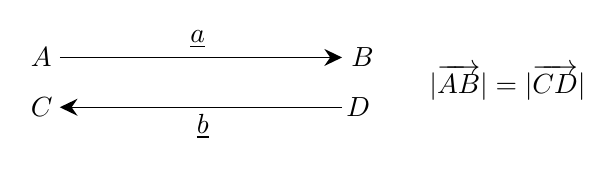
\begin{tikzpicture}[x=0.75pt,y=0.75pt,yscale=-0.8,xscale=0.8]
%uncomment if require: \path (0,179); %set diagram left start at 0, and has height of 179

%Straight Lines [id:da4122672604500781] 
\draw    (220,80) -- (387,80) ;
\draw [shift={(390,80)}, rotate = 180] [fill={rgb, 255:red, 0; green, 0; blue, 0 }  ][line width=0.08]  [draw opacity=0] (10.72,-5.15) -- (0,0) -- (10.72,5.15) -- (7.12,0) -- cycle    ;
%Straight Lines [id:da2306946235955416] 
\draw    (390,110) -- (223,110) ;
\draw [shift={(220,110)}, rotate = 360] [fill={rgb, 255:red, 0; green, 0; blue, 0 }  ][line width=0.08]  [draw opacity=0] (10.72,-5.15) -- (0,0) -- (10.72,5.15) -- (7.12,0) -- cycle    ;

% Text Node
\draw (201,72.4) node [anchor=north west][inner sep=0.75pt]    {$A$};
% Text Node
\draw (301,112.4) node [anchor=north west][inner sep=0.75pt]    {$\underline{b}$};
% Text Node
\draw (297,62.4) node [anchor=north west][inner sep=0.75pt]    {$\underline{a}$};
% Text Node
\draw (391,102.4) node [anchor=north west][inner sep=0.75pt]    {$D$};
% Text Node
\draw (201,102.4) node [anchor=north west][inner sep=0.75pt]    {$C$};
% Text Node
\draw (394,72.4) node [anchor=north west][inner sep=0.75pt]    {$B$};
% Text Node
\draw (441,82.4) node [anchor=north west][inner sep=0.75pt]    {$|\overrightarrow{AB}|=|\overrightarrow{CD}|$};


\end{tikzpicture}
		\caption{Opposite Vector}
		\label{vec-fig-4}
	\end{figure}
	চিত্র \ref{vec-fig-4} এ $\overrightarrow{AB}=-\overrightarrow{CD}$
	
	\newpage
	\item \textbf{সমতলীয় ভেক্টর (Coplanar Vectors):} কতগুলো ভেক্টরকে সমতলীয় বলা হয়, যদি তাদের ধারক রেখা অভিন্ন সমতলের সমান্তরাল হয়।
	
	\item \textbf{অবস্থান ভেক্টর (Position Vector):} স্থির প্রসঙ্গ কাঠামো ও মূলবিন্দুর সাপেক্ষে কোনো বিন্দুর অবস্থান নির্দেশক ভেক্টরকে অবস্থান ভেক্টর বলে। চিত্র \ref{vec-fig-5} এ $P$ বিন্দুর অবস্থান ভেক্টর $\underline{r}$। অর্থাৎ $\overrightarrow{OP}=\underline{r}$ বা $P(\underline{r})$। 
	\begin{figure}[h]
		\centering
		

\tikzset{every picture/.style={line width=0.75pt}} %set default line width to 0.75pt        

\begin{tikzpicture}[x=0.75pt,y=0.75pt,yscale=-0.8,xscale=0.8]
%uncomment if require: \path (0,300); %set diagram left start at 0, and has height of 300

%Shape: Axis 2D [id:dp15761041967637524] 
\draw  (150,228.4) -- (335.5,228.4)(168.55,70) -- (168.55,246) (328.5,223.4) -- (335.5,228.4) -- (328.5,233.4) (163.55,77) -- (168.55,70) -- (173.55,77)  ;
%Straight Lines [id:da5719661880478002] 
\draw    (168.55,228.4) -- (257.96,132.2) ;
\draw [shift={(260,130)}, rotate = 492.9] [fill={rgb, 255:red, 0; green, 0; blue, 0 }  ][line width=0.08]  [draw opacity=0] (8.93,-4.29) -- (0,0) -- (8.93,4.29) -- cycle    ;

% Text Node
\draw (151,232.4) node [anchor=north west][inner sep=0.75pt]    {$O$};
% Text Node
\draw (261,112.4) node [anchor=north west][inner sep=0.75pt]    {$P$};
% Text Node
\draw (161,52.4) node [anchor=north west][inner sep=0.75pt]    {$Y$};
% Text Node
\draw (341,222.4) node [anchor=north west][inner sep=0.75pt]    {$X$};
% Text Node
\draw (201,162.4) node [anchor=north west][inner sep=0.75pt]    {$\underline{r}$};


\end{tikzpicture}
		\caption{Position Vector}
		\label{vec-fig-5}
	\end{figure}

	\item \textbf{ভেক্টরের যোগাশ্রয়ী সমাবেশ (Linear Combination of Vectors):}\\ কোনো ভেক্টর $\underline{r}$ কে $\underline{v_1}, \underline{v_2}, \cdots, \underline{v_n}$ ভেক্তরগুলির যোগাশ্রয়ী সমাবেশ বলা হয় যদি\\ $\underline{r}=\alpha_1\underline{v_1}+\alpha_2\underline{v_2}+\cdots+\alpha_n\underline{v_n}$ হয়। যেখানে $\alpha_1, \alpha_2, \cdots, \alpha_n$ স্কেলার রাশি। 
\end{enumerate}
\newpage
\section*{দুইটি ভেক্টরের অন্তর্ভুক্ত কোণ \\(Angle Between Two Vectors)}
\begin{figure}[h]
	\centering
	

\tikzset{every picture/.style={line width=0.75pt}} %set default line width to 0.75pt        

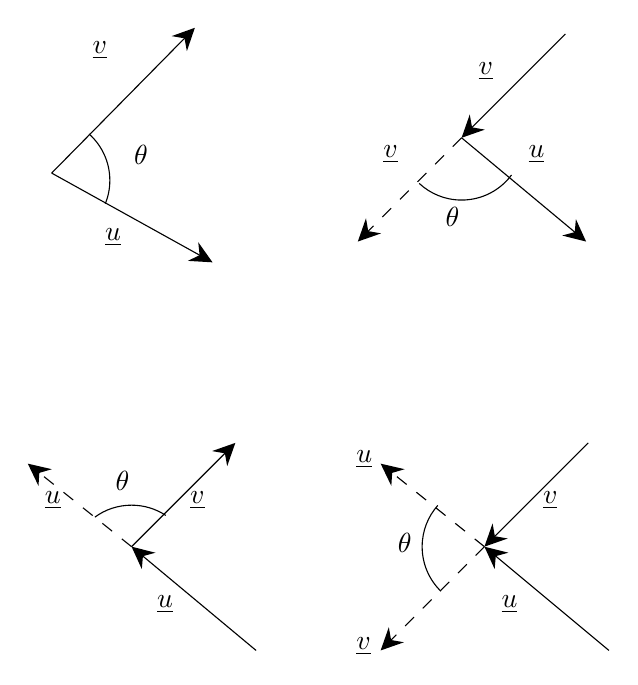
\begin{tikzpicture}[x=0.75pt,y=0.75pt,yscale=-1,xscale=1]
%uncomment if require: \path (0,419); %set diagram left start at 0, and has height of 419

%Straight Lines [id:da12880106894913612] 
\draw    (203.5,127) -- (270.39,59.14) ;
\draw [shift={(272.5,57)}, rotate = 494.59] [fill={rgb, 255:red, 0; green, 0; blue, 0 }  ][line width=0.08]  [draw opacity=0] (10.72,-5.15) -- (0,0) -- (10.72,5.15) -- (7.12,0) -- cycle    ;
%Straight Lines [id:da4719340618715049] 
\draw    (203.5,127) -- (278.38,168.54) ;
\draw [shift={(281,170)}, rotate = 209.02] [fill={rgb, 255:red, 0; green, 0; blue, 0 }  ][line width=0.08]  [draw opacity=0] (10.72,-5.15) -- (0,0) -- (10.72,5.15) -- (7.12,0) -- cycle    ;
%Straight Lines [id:da7782548290653029] 
\draw    (451,60) -- (403.12,107.88) ;
\draw [shift={(401,110)}, rotate = 315] [fill={rgb, 255:red, 0; green, 0; blue, 0 }  ][line width=0.08]  [draw opacity=0] (10.72,-5.15) -- (0,0) -- (10.72,5.15) -- (7.12,0) -- cycle    ;
%Straight Lines [id:da054039739072695436] 
\draw    (401,110) -- (458.7,158.08) ;
\draw [shift={(461,160)}, rotate = 219.81] [fill={rgb, 255:red, 0; green, 0; blue, 0 }  ][line width=0.08]  [draw opacity=0] (10.72,-5.15) -- (0,0) -- (10.72,5.15) -- (7.12,0) -- cycle    ;
%Straight Lines [id:da11490224320825582] 
\draw  [dash pattern={on 4.5pt off 4.5pt}]  (401,110) -- (353.12,157.88) ;
\draw [shift={(351,160)}, rotate = 315] [fill={rgb, 255:red, 0; green, 0; blue, 0 }  ][line width=0.08]  [draw opacity=0] (10.72,-5.15) -- (0,0) -- (10.72,5.15) -- (7.12,0) -- cycle    ;
%Straight Lines [id:da6544357034582597] 
\draw    (242,307) -- (289.88,259.12) ;
\draw [shift={(292,257)}, rotate = 495] [fill={rgb, 255:red, 0; green, 0; blue, 0 }  ][line width=0.08]  [draw opacity=0] (10.72,-5.15) -- (0,0) -- (10.72,5.15) -- (7.12,0) -- cycle    ;
%Straight Lines [id:da3827614521360492] 
\draw    (302,357) -- (244.3,308.92) ;
\draw [shift={(242,307)}, rotate = 399.81] [fill={rgb, 255:red, 0; green, 0; blue, 0 }  ][line width=0.08]  [draw opacity=0] (10.72,-5.15) -- (0,0) -- (10.72,5.15) -- (7.12,0) -- cycle    ;
%Straight Lines [id:da20364987214219643] 
\draw  [dash pattern={on 4.5pt off 4.5pt}]  (242,307) -- (194.34,268.87) ;
\draw [shift={(192,267)}, rotate = 398.65999999999997] [fill={rgb, 255:red, 0; green, 0; blue, 0 }  ][line width=0.08]  [draw opacity=0] (10.72,-5.15) -- (0,0) -- (10.72,5.15) -- (7.12,0) -- cycle    ;
%Straight Lines [id:da7168909647979127] 
\draw    (462,257) -- (414.12,304.88) ;
\draw [shift={(412,307)}, rotate = 315] [fill={rgb, 255:red, 0; green, 0; blue, 0 }  ][line width=0.08]  [draw opacity=0] (10.72,-5.15) -- (0,0) -- (10.72,5.15) -- (7.12,0) -- cycle    ;
%Straight Lines [id:da026059643406870947] 
\draw    (472,357) -- (414.3,308.92) ;
\draw [shift={(412,307)}, rotate = 399.81] [fill={rgb, 255:red, 0; green, 0; blue, 0 }  ][line width=0.08]  [draw opacity=0] (10.72,-5.15) -- (0,0) -- (10.72,5.15) -- (7.12,0) -- cycle    ;
%Straight Lines [id:da13860947747573515] 
\draw  [dash pattern={on 4.5pt off 4.5pt}]  (412,307) -- (364.12,354.88) ;
\draw [shift={(362,357)}, rotate = 315] [fill={rgb, 255:red, 0; green, 0; blue, 0 }  ][line width=0.08]  [draw opacity=0] (10.72,-5.15) -- (0,0) -- (10.72,5.15) -- (7.12,0) -- cycle    ;
%Straight Lines [id:da8944641852155986] 
\draw  [dash pattern={on 4.5pt off 4.5pt}]  (412,307) -- (364.34,268.87) ;
\draw [shift={(362,267)}, rotate = 398.65999999999997] [fill={rgb, 255:red, 0; green, 0; blue, 0 }  ][line width=0.08]  [draw opacity=0] (10.72,-5.15) -- (0,0) -- (10.72,5.15) -- (7.12,0) -- cycle    ;
%Shape: Arc [id:dp13134117459212136] 
\draw  [draw opacity=0] (425.06,127.93) .. controls (419.59,135.25) and (410.85,140) .. (401,140) .. controls (393.11,140) and (385.94,136.96) .. (380.59,131.98) -- (401,110) -- cycle ; \draw   (425.06,127.93) .. controls (419.59,135.25) and (410.85,140) .. (401,140) .. controls (393.11,140) and (385.94,136.96) .. (380.59,131.98) ;
%Shape: Arc [id:dp3092789865341268] 
\draw  [draw opacity=0] (221.55,108.18) .. controls (227.67,113.67) and (231.53,121.64) .. (231.53,130.52) .. controls (231.53,134.48) and (230.76,138.27) .. (229.36,141.74) -- (201.53,130.52) -- cycle ; \draw   (221.55,108.18) .. controls (227.67,113.67) and (231.53,121.64) .. (231.53,130.52) .. controls (231.53,134.48) and (230.76,138.27) .. (229.36,141.74) ;
%Shape: Arc [id:dp9907407736423404] 
\draw  [draw opacity=0] (224.32,292.76) .. controls (229.28,289.14) and (235.39,287) .. (242,287) .. controls (248.11,287) and (253.79,288.82) .. (258.52,291.96) -- (242,317) -- cycle ; \draw   (224.32,292.76) .. controls (229.28,289.14) and (235.39,287) .. (242,287) .. controls (248.11,287) and (253.79,288.82) .. (258.52,291.96) ;
%Shape: Arc [id:dp2992175381309219] 
\draw  [draw opacity=0] (391.04,328.47) .. controls (385.46,323.02) and (382,315.41) .. (382,307) .. controls (382,299.38) and (384.84,292.42) .. (389.52,287.13) -- (412,307) -- cycle ; \draw   (391.04,328.47) .. controls (385.46,323.02) and (382,315.41) .. (382,307) .. controls (382,299.38) and (384.84,292.42) .. (389.52,287.13) ;

% Text Node
\draw (228,152.4) node [anchor=north west][inner sep=0.75pt]    {$\underline{u}$};
% Text Node
\draw (222,62.4) node [anchor=north west][inner sep=0.75pt]    {$\underline{v}$};
% Text Node
\draw (432,112.4) node [anchor=north west][inner sep=0.75pt]    {$\underline{u}$};
% Text Node
\draw (362,112.4) node [anchor=north west][inner sep=0.75pt]    {$\underline{v}$};
% Text Node
\draw (408,72.4) node [anchor=north west][inner sep=0.75pt]    {$\underline{v}$};
% Text Node
\draw (253,329.4) node [anchor=north west][inner sep=0.75pt]    {$\underline{u}$};
% Text Node
\draw (199,279.4) node [anchor=north west][inner sep=0.75pt]    {$\underline{u}$};
% Text Node
\draw (419,329.4) node [anchor=north west][inner sep=0.75pt]    {$\underline{u}$};
% Text Node
\draw (349,259.4) node [anchor=north west][inner sep=0.75pt]    {$\underline{u}$};
% Text Node
\draw (269,279.4) node [anchor=north west][inner sep=0.75pt]    {$\underline{v}$};
% Text Node
\draw (439,279.4) node [anchor=north west][inner sep=0.75pt]    {$\underline{v}$};
% Text Node
\draw (349,349.4) node [anchor=north west][inner sep=0.75pt]    {$\underline{v}$};
% Text Node
\draw (242,112.4) node [anchor=north west][inner sep=0.75pt]    {$\theta $};
% Text Node
\draw (392,142.4) node [anchor=north west][inner sep=0.75pt]    {$\theta $};
% Text Node
\draw (233,269.4) node [anchor=north west][inner sep=0.75pt]    {$\theta $};
% Text Node
\draw (369,299.4) node [anchor=north west][inner sep=0.75pt]    {$\theta $};


\end{tikzpicture}
	\caption{দুইটি ভেক্টরের অন্তর্ভুক্ত কোণ}
	\label{vec-fig-6}
\end{figure}
মনেকরি $\underline{u}$ ও $\underline{v}$ ভেক্টর দুইটি একটি নির্দিষ্ট বিন্দুতে ছেদ করেছে। তাদের অন্তর্ভুক্ত কোণ $\theta$ হলে $0\leq\theta\leq\pi$। (চিত্র \ref{vec-fig-6})।   
\begin{tcolorbox}
	\textbf{Note:} দুইটি ভেক্টরের অন্তর্ভুক্ত কোণ মাপার সময় অবশ্যই ভেক্টর দুইটির আদিবিন্দু অথবা অন্তবিন্দু একই বিন্দুতে মিলিত হতে হবে। 
\end{tcolorbox}
\section*{ভেক্টর সংক্রান্ত সূত্রসমূহ (Law's of Vector)}
\subsection*{ভেক্টর যোগের ত্রিভুজ সূত্র (Triangle Law of Addition)}
\begin{tcolorbox}[colback=green!5!white,colframe=green!75!black,title=ত্রিভুজ সূত্র]
	কোনো ভেক্টর $\underline{u}$ এর প্রান্তবিন্দু হতে অপর একটি ভেক্টর $\underline{v}$ অঙ্কন করা হলে $\underline{u}+\underline{v}$ দ্বারা এরুপ একটি ভেক্টর বোঝায় যার আদিবিন্দু $\underline{u}$ এর আদিবিন্দু এবং যার প্রান্তবিন্দু $\underline{v}$ এর প্রান্তবিন্দু।
\end{tcolorbox}
\begin{figure}[h]
	\centering
	

\tikzset{every picture/.style={line width=0.75pt}} %set default line width to 0.75pt        

\begin{tikzpicture}[x=0.75pt,y=0.75pt,yscale=-0.9,xscale=0.9]
%uncomment if require: \path (0,300); %set diagram left start at 0, and has height of 300

%Straight Lines [id:da3683399638260374] 
\draw    (200,180) -- (367,180) ;
\draw [shift={(370,180)}, rotate = 180] [fill={rgb, 255:red, 0; green, 0; blue, 0 }  ][line width=0.08]  [draw opacity=0] (10.72,-5.15) -- (0,0) -- (10.72,5.15) -- (7.12,0) -- cycle    ;
%Straight Lines [id:da012426198552259127] 
\draw    (370,180) -- (457.99,82.23) ;
\draw [shift={(460,80)}, rotate = 491.99] [fill={rgb, 255:red, 0; green, 0; blue, 0 }  ][line width=0.08]  [draw opacity=0] (10.72,-5.15) -- (0,0) -- (10.72,5.15) -- (7.12,0) -- cycle    ;
%Straight Lines [id:da507431700036358] 
\draw    (200,180) -- (460,80) ;
\draw  [fill={rgb, 255:red, 0; green, 0; blue, 0 }  ,fill opacity=1 ] (330.64,123.53) -- (341.77,124.68) -- (334.18,132.89) ;

% Text Node
\draw (181,182.4) node [anchor=north west][inner sep=0.75pt]    {$O$};
% Text Node
\draw (372,183.4) node [anchor=north west][inner sep=0.75pt]    {$A$};
% Text Node
\draw (461,62.4) node [anchor=north west][inner sep=0.75pt]    {$B$};
% Text Node
\draw (274,182.4) node [anchor=north west][inner sep=0.75pt]    {$\underline{u}$};
% Text Node
\draw (301.81,106.57) node [anchor=north west][inner sep=0.75pt]  [rotate=-338.43]  {$\underline{u} +\underline{v}$};
% Text Node
\draw (414,132.4) node [anchor=north west][inner sep=0.75pt]    {$\underline{v}$};


\end{tikzpicture}
	\caption{ত্রিভুজ সূত্র}
	\label{vec-fig-7}
\end{figure} 

\subsection*{ভেক্টর যোগের সামান্তরিক সূত্র (Parallelogram Law of Addition)}
\begin{tcolorbox}[colback=green!5!white,colframe=green!75!black,title=সামান্তরিক সূত্র]
	ভেক্টর $\underline{u}$ ও $\underline{v}$ কে একটি সামান্তরিকের দুইটি সন্নিহিত বাহু দ্বারা মানে ও দিকে সূচিত করা হলে, ভেক্তরদয়ের ছেদবিন্দুগামি সামান্তরিকের কর্ণটি ভেক্ত্ররদয়ের লব্ধি $\underline{u}+\underline{v}$ কে মানে ও দিকে প্রকাশ করবে।
\end{tcolorbox}
\begin{figure}[h]
	\centering
	

\tikzset{every picture/.style={line width=0.75pt}} %set default line width to 0.75pt        

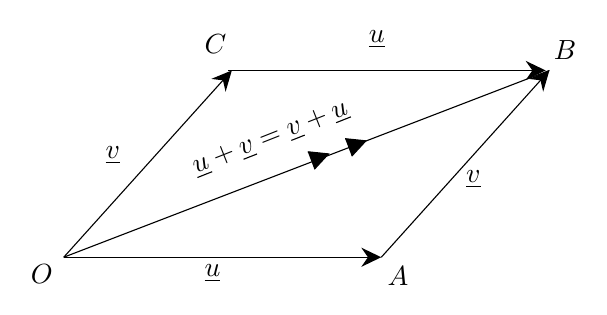
\begin{tikzpicture}[x=0.75pt,y=0.75pt,yscale=-0.9,xscale=0.9]
%uncomment if require: \path (0,365); %set diagram left start at 0, and has height of 365

%Straight Lines [id:da29745656361417705] 
\draw    (220,200) -- (387,200) ;
\draw [shift={(390,200)}, rotate = 180] [fill={rgb, 255:red, 0; green, 0; blue, 0 }  ][line width=0.08]  [draw opacity=0] (10.72,-5.15) -- (0,0) -- (10.72,5.15) -- (7.12,0) -- cycle    ;
%Straight Lines [id:da49149583208157477] 
\draw    (390,200) -- (477.99,102.23) ;
\draw [shift={(480,100)}, rotate = 491.99] [fill={rgb, 255:red, 0; green, 0; blue, 0 }  ][line width=0.08]  [draw opacity=0] (10.72,-5.15) -- (0,0) -- (10.72,5.15) -- (7.12,0) -- cycle    ;
%Straight Lines [id:da41358510781009916] 
\draw    (220,200) -- (480,100) ;
\draw  [fill={rgb, 255:red, 0; green, 0; blue, 0 }  ,fill opacity=1 ] (350.64,143.53) -- (361.77,144.68) -- (354.18,152.89) ;
%Straight Lines [id:da8720803166983586] 
\draw    (220,200) -- (307.99,102.23) ;
\draw [shift={(310,100)}, rotate = 491.99] [fill={rgb, 255:red, 0; green, 0; blue, 0 }  ][line width=0.08]  [draw opacity=0] (10.72,-5.15) -- (0,0) -- (10.72,5.15) -- (7.12,0) -- cycle    ;
%Straight Lines [id:da772741802301026] 
\draw    (308,100) -- (475,100) ;
\draw [shift={(478,100)}, rotate = 180] [fill={rgb, 255:red, 0; green, 0; blue, 0 }  ][line width=0.08]  [draw opacity=0] (10.72,-5.15) -- (0,0) -- (10.72,5.15) -- (7.12,0) -- cycle    ;
\draw  [fill={rgb, 255:red, 0; green, 0; blue, 0 }  ,fill opacity=1 ] (370.64,136.53) -- (381.77,137.68) -- (374.18,145.89) ;

% Text Node
\draw (201,202.4) node [anchor=north west][inner sep=0.75pt]    {$O$};
% Text Node
\draw (392,203.4) node [anchor=north west][inner sep=0.75pt]    {$A$};
% Text Node
\draw (481,82.4) node [anchor=north west][inner sep=0.75pt]    {$B$};
% Text Node
\draw (294,202.4) node [anchor=north west][inner sep=0.75pt]    {$\underline{u}$};
% Text Node
\draw (285.81,146.57) node [anchor=north west][inner sep=0.75pt]  [rotate=-338.43]  {$\underline{u} +\underline{v} =\underline{v} +\underline{u}$};
% Text Node
\draw (434,152.4) node [anchor=north west][inner sep=0.75pt]    {$\underline{v}$};
% Text Node
\draw (241,139.4) node [anchor=north west][inner sep=0.75pt]    {$\underline{v}$};
% Text Node
\draw (382,77.4) node [anchor=north west][inner sep=0.75pt]    {$\underline{u}$};
% Text Node
\draw (294,79.4) node [anchor=north west][inner sep=0.75pt]    {$C$};


\end{tikzpicture}
	\caption{সামান্তরিক সূত্র}
	\label{vec-fig-8}
\end{figure} 

\subsection*{অন্তর্বিভক্তিকরণ সূত্র}
\begin{tcolorbox}[colback=green!5!white,colframe=green!75!black]
	$A, B, C$ এর অবস্থান ভেক্টর যথাক্রমে $\underline{a}, \underline{b}, \underline{c}$ হলে এবং $C$ বিন্দু $AB$ রেখাংশকে $m:n$ অনুপাতে অন্তর্বিভক্ত করলে $\underline{c}=\dfrac{m\underline{b}+n\underline{a}}{m+n}$
\end{tcolorbox}
\begin{wrapfigure}[5]{r}{0.5\textwidth}
	\begin{center}
		

\tikzset{every picture/.style={line width=0.75pt}} %set default line width to 0.75pt        

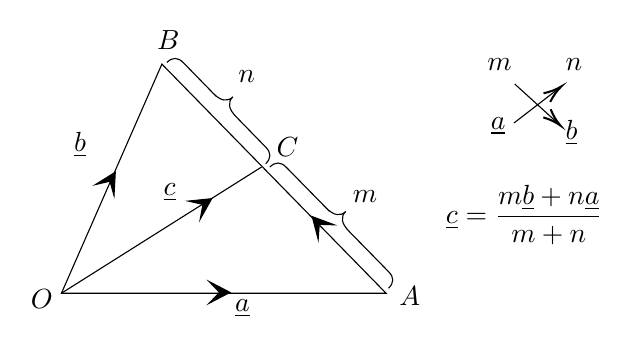
\begin{tikzpicture}[x=0.75pt,y=0.75pt,yscale=-0.8,xscale=0.8]
%uncomment if require: \path (0,300); %set diagram left start at 0, and has height of 300

%Shape: Triangle [id:dp7803720964557852] 
\draw   (218.5,70) -- (353.5,208) -- (158,208) -- cycle ;
\draw  [fill={rgb, 255:red, 0; green, 0; blue, 0 }  ,fill opacity=1 ] (247,201) -- (259.5,207.5) -- (247,214) -- (253.25,207.5) -- cycle ;
\draw  [fill={rgb, 255:red, 0; green, 0; blue, 0 }  ,fill opacity=1 ] (178.47,142.57) -- (190.43,135.12) -- (189.66,149.19) -- (187.25,140.5) -- cycle ;
%Straight Lines [id:da7513488205154673] 
\draw    (158,208) -- (278.5,132) ;
\draw  [fill={rgb, 255:red, 0; green, 0; blue, 0 }  ,fill opacity=1 ] (234.46,152.5) -- (248.47,151.07) -- (241.59,163.36) -- (243.25,154.5) -- cycle ;
%Shape: Brace [id:dp6937774928119653] 
\draw   (281,130) .. controls (284.34,126.74) and (284.38,123.44) .. (281.12,120.1) -- (263.24,101.77) .. controls (258.59,97) and (257.93,92.98) .. (261.27,89.73) .. controls (257.93,92.98) and (253.93,92.23) .. (249.28,87.46)(251.37,89.6) -- (231.4,69.13) .. controls (228.14,65.79) and (224.84,65.75) .. (221.5,69) ;
%Shape: Brace [id:dp9394696690029762] 
\draw   (355,205) .. controls (358.33,201.73) and (358.37,198.43) .. (355.1,195.1) -- (331.25,170.75) .. controls (326.58,165.98) and (325.92,161.97) .. (329.25,158.71) .. controls (325.92,161.97) and (321.92,161.22) .. (317.25,156.46)(319.35,158.6) -- (293.39,132.11) .. controls (290.12,128.78) and (286.82,128.74) .. (283.49,132.01) ;
\draw  [fill={rgb, 255:red, 0; green, 0; blue, 0 }  ,fill opacity=1 ] (312.62,175.5) -- (309.06,161.86) -- (322.26,166.78) -- (313.25,166.5) -- cycle ;
%Straight Lines [id:da7583773908360483] 
\draw    (431,82) -- (457.02,105.65) ;
\draw [shift={(458.5,107)}, rotate = 222.27] [color={rgb, 255:red, 0; green, 0; blue, 0 }  ][line width=0.75]    (10.93,-3.29) .. controls (6.95,-1.4) and (3.31,-0.3) .. (0,0) .. controls (3.31,0.3) and (6.95,1.4) .. (10.93,3.29)   ;
%Straight Lines [id:da19534068791687043] 
\draw    (430.5,105.5) -- (457.42,84.72) ;
\draw [shift={(459,83.5)}, rotate = 502.33] [color={rgb, 255:red, 0; green, 0; blue, 0 }  ][line width=0.75]    (10.93,-3.29) .. controls (6.95,-1.4) and (3.31,-0.3) .. (0,0) .. controls (3.31,0.3) and (6.95,1.4) .. (10.93,3.29)   ;

% Text Node
\draw (138,204.4) node [anchor=north west][inner sep=0.75pt]    {$O$};
% Text Node
\draw (360,202.4) node [anchor=north west][inner sep=0.75pt]    {$A$};
% Text Node
\draw (214,48.4) node [anchor=north west][inner sep=0.75pt]    {$B$};
% Text Node
\draw (261,210.4) node [anchor=north west][inner sep=0.75pt]    {$\underline{a}$};
% Text Node
\draw (164,109.4) node [anchor=north west][inner sep=0.75pt]    {$\underline{b}$};
% Text Node
\draw (218,140.4) node [anchor=north west][inner sep=0.75pt]    {$\underline{c}$};
% Text Node
\draw (286,112.4) node [anchor=north west][inner sep=0.75pt]    {$C$};
% Text Node
\draw (263,72.4) node [anchor=north west][inner sep=0.75pt]    {$n$};
% Text Node
\draw (332,144.4) node [anchor=north west][inner sep=0.75pt]    {$m$};
% Text Node
\draw (388,141.4) node [anchor=north west][inner sep=0.75pt]    {$\underline{c} =\dfrac{m\underline{b} +n\underline{a}}{m+n}$};
% Text Node
\draw (413,65.4) node [anchor=north west][inner sep=0.75pt]    {$m$};
% Text Node
\draw (460,65.4) node [anchor=north west][inner sep=0.75pt]    {$n$};
% Text Node
\draw (415,100.4) node [anchor=north west][inner sep=0.75pt]    {$\underline{a}$};
% Text Node
\draw (460,102.4) node [anchor=north west][inner sep=0.75pt]    {$\underline{b}$};


\end{tikzpicture}
	\end{center}
	\caption{অন্তর্বিভক্তিকরণ সূত্র}
	\label{vec-fig-9}
\end{wrapfigure}
\textbf{প্রমাণঃ} দেওয়া আছে, 
\begin{align*}
	AC:BC &= m:n \\
	\Rightarrow \dfrac{AC}{BC} &= \dfrac{m}{n} \\
	\Rightarrow \dfrac{AC}{AC+BC} &= \dfrac{m}{m+n} \\
	\Rightarrow \dfrac{AC}{AB} &= \dfrac{m}{m+n} \\
	\therefore AC &= \dfrac{m}{m+n} AB \\
	\therefore \overrightarrow{AC} &= \dfrac{m}{m+n} \overrightarrow{AB} \\
	\Rightarrow \overrightarrow{AC} &= \dfrac{m}{m+n} (\overrightarrow{OB}-\overrightarrow{OA}) \quad \quad [\because \overrightarrow{OA}+\overrightarrow{AB}=\overrightarrow{OB}]
\end{align*}
\begin{equation}
	\therefore \overrightarrow{AC} = \dfrac{m}{m+n} (\underline{b}-\underline{a}) \tag{1}
\end{equation}
$\triangle OAC$ হতে পাই, 
\begin{align*}
	\overrightarrow{OA}+\overrightarrow{AC} &= \overrightarrow{OC} \\
	\Rightarrow \underline{a}+\dfrac{m}{m+n} (\underline{b}-\underline{a}) &= \underline{c} \quad \quad [\because \text{(1) হতে}]\\
	\Rightarrow \underline{c} &= \dfrac{m(\underline{b}-\underline{a})+(m+n)\underline{a}}{m+n}\\
	\Rightarrow \underline{c} &= \dfrac{m\underline{b}+(m+n-m)\underline{a}}{m+n} \\
	\therefore \underline{c} &= \dfrac{m\underline{b}+n\underline{a}}{m+n}
\end{align*}
\newpage
\subsection*{বহির্বিভক্তিকরণ সূত্র}
\begin{tcolorbox}[colback=green!5!white,colframe=green!75!black]
	$A, B, C$ এর অবস্থান ভেক্টর যথাক্রমে $\underline{a}, \underline{b}, \underline{c}$ হলে এবং $C$ বিন্দু $AB$ রেখাংশকে $m:n$ অনুপাতে বহির্বিভক্ত করলে $\underline{c}=\dfrac{m\underline{b}-n\underline{a}}{m-n}$
\end{tcolorbox}
\begin{wrapfigure}[5]{r}{0.5\textwidth}
	\begin{center}
		

\tikzset{every picture/.style={line width=0.75pt}} %set default line width to 0.75pt        

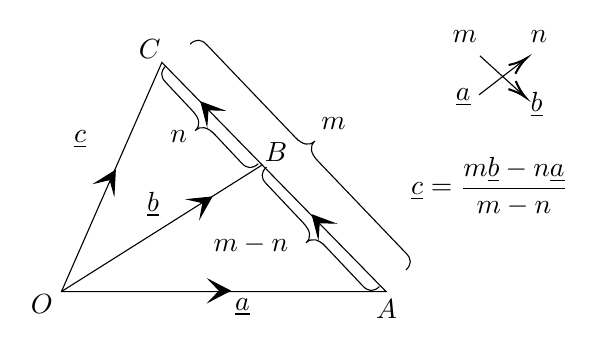
\begin{tikzpicture}[x=0.75pt,y=0.75pt,yscale=-0.8,xscale=0.8]
%uncomment if require: \path (0,300); %set diagram left start at 0, and has height of 300

%Shape: Triangle [id:dp6057132058653998] 
\draw   (265.5,90) -- (400.5,228) -- (205,228) -- cycle ;
\draw  [fill={rgb, 255:red, 0; green, 0; blue, 0 }  ,fill opacity=1 ] (294,221) -- (306.5,227.5) -- (294,234) -- (300.25,227.5) -- cycle ;
\draw  [fill={rgb, 255:red, 0; green, 0; blue, 0 }  ,fill opacity=1 ] (225.47,162.57) -- (237.43,155.12) -- (236.66,169.19) -- (234.25,160.5) -- cycle ;
%Straight Lines [id:da5161540821426658] 
\draw    (205,228) -- (325.5,152) ;
\draw  [fill={rgb, 255:red, 0; green, 0; blue, 0 }  ,fill opacity=1 ] (281.46,172.5) -- (295.47,171.07) -- (288.59,183.36) -- (290.25,174.5) -- cycle ;
%Shape: Brace [id:dp2907792729734002] 
\draw   (268,92) .. controls (264.6,95.2) and (264.5,98.5) .. (267.7,101.89) -- (283.8,119.01) .. controls (288.37,123.87) and (288.95,127.9) .. (285.55,131.09) .. controls (288.95,127.9) and (292.93,128.73) .. (297.5,133.58)(295.45,131.39) -- (313.61,150.7) .. controls (316.8,154.1) and (320.1,154.2) .. (323.5,151) ;
%Shape: Brace [id:dp31460660756332137] 
\draw   (412.5,215) .. controls (415.87,211.77) and (415.95,208.47) .. (412.72,205.1) -- (359.47,149.39) .. controls (354.86,144.58) and (354.25,140.56) .. (357.62,137.33) .. controls (354.25,140.56) and (350.26,139.76) .. (345.65,134.94)(347.72,137.11) -- (292.39,79.23) .. controls (289.16,75.86) and (285.86,75.78) .. (282.49,79) ;
\draw  [fill={rgb, 255:red, 0; green, 0; blue, 0 }  ,fill opacity=1 ] (359.62,195.5) -- (356.06,181.86) -- (369.26,186.78) -- (360.25,186.5) -- cycle ;
%Shape: Brace [id:dp8011846743806035] 
\draw   (328.5,153) .. controls (325.11,156.21) and (325.01,159.51) .. (328.22,162.9) -- (350.54,186.54) .. controls (355.12,191.39) and (355.71,195.41) .. (352.32,198.61) .. controls (355.71,195.41) and (359.7,196.23) .. (364.27,201.08)(362.21,198.9) -- (386.6,224.72) .. controls (389.81,228.11) and (393.11,228.21) .. (396.5,225) ;
%Straight Lines [id:da6231155430584114] 
\draw    (457,86) -- (483.02,109.65) ;
\draw [shift={(484.5,111)}, rotate = 222.27] [color={rgb, 255:red, 0; green, 0; blue, 0 }  ][line width=0.75]    (10.93,-3.29) .. controls (6.95,-1.4) and (3.31,-0.3) .. (0,0) .. controls (3.31,0.3) and (6.95,1.4) .. (10.93,3.29)   ;
%Straight Lines [id:da6271046257844906] 
\draw    (456.5,109.5) -- (483.42,88.72) ;
\draw [shift={(485,87.5)}, rotate = 502.33] [color={rgb, 255:red, 0; green, 0; blue, 0 }  ][line width=0.75]    (10.93,-3.29) .. controls (6.95,-1.4) and (3.31,-0.3) .. (0,0) .. controls (3.31,0.3) and (6.95,1.4) .. (10.93,3.29)   ;
\draw  [fill={rgb, 255:red, 0; green, 0; blue, 0 }  ,fill opacity=1 ] (292.62,127.5) -- (289.06,113.86) -- (302.26,118.78) -- (293.25,118.5) -- cycle ;

% Text Node
\draw (185,228.4) node [anchor=north west][inner sep=0.75pt]    {$O$};
% Text Node
\draw (393,231.4) node [anchor=north west][inner sep=0.75pt]    {$A$};
% Text Node
\draw (250,74.4) node [anchor=north west][inner sep=0.75pt]    {$C$};
% Text Node
\draw (308,230.4) node [anchor=north west][inner sep=0.75pt]    {$\underline{a}$};
% Text Node
\draw (211,129.4) node [anchor=north west][inner sep=0.75pt]    {$\underline{c}$};
% Text Node
\draw (255,166.4) node [anchor=north west][inner sep=0.75pt]    {$\underline{b}$};
% Text Node
\draw (326,136.4) node [anchor=north west][inner sep=0.75pt]    {$B$};
% Text Node
\draw (269,129.4) node [anchor=north west][inner sep=0.75pt]    {$n$};
% Text Node
\draw (360,121.4) node [anchor=north west][inner sep=0.75pt]    {$m$};
% Text Node
\draw (295,192.4) node [anchor=north west][inner sep=0.75pt]    {$m-n$};
% Text Node
\draw (414,145.4) node [anchor=north west][inner sep=0.75pt]    {$\underline{c} =\dfrac{m\underline{b} -n\underline{a}}{m-n}$};
% Text Node
\draw (439,69.4) node [anchor=north west][inner sep=0.75pt]    {$m$};
% Text Node
\draw (486,69.4) node [anchor=north west][inner sep=0.75pt]    {$n$};
% Text Node
\draw (441,104.4) node [anchor=north west][inner sep=0.75pt]    {$\underline{a}$};
% Text Node
\draw (486,106.4) node [anchor=north west][inner sep=0.75pt]    {$\underline{b}$};


\end{tikzpicture}
	\end{center}
	\caption{বহির্বিভক্তিকরণ সূত্র}
	\label{vec-fig-10}
\end{wrapfigure}
\textbf{প্রমাণঃ} দেওয়া আছে, 
\begin{align*}
	AC:BC &= m:n \\
	\Rightarrow \dfrac{AC}{BC} &= \dfrac{m}{n} \\
	\Rightarrow \dfrac{AC-BC}{BC} &= \dfrac{m-n}{n} \\
	\Rightarrow \dfrac{AB}{BC} &= \dfrac{m-n}{n} \\
	\therefore BC &= \dfrac{n}{m-n}AB \\
	\therefore \overrightarrow{BC} &= \dfrac{n}{m-n}\overrightarrow{AB} \\
	\Rightarrow \overrightarrow{BC} &= \dfrac{n}{m-n}(\overrightarrow{OB}-\overrightarrow{OA}) \quad \quad [\because \overrightarrow{OA}+\overrightarrow{AB}=\overrightarrow{OB}]
\end{align*}
\begin{equation}
	\therefore \overrightarrow{BC} = \dfrac{n}{m-n}(\underline{b}-\underline{a}) \tag{1}
\end{equation}
$\triangle OBC$ হতে পাই,
\begin{align*}
	\overrightarrow{OB}+\overrightarrow{BC} &= \overrightarrow{OC} \\
	\Rightarrow \underline{b}+\dfrac{n}{m-n}(\underline{b}-\underline{a}) &= \underline{c} \quad \quad [\because \text{(1) হতে}]\\
	\Rightarrow \underline{c} &= \dfrac{(m-n)\underline{b}+n(\underline{b}-\underline{a})}{m-n} \\
	\Rightarrow \underline{c} &= \dfrac{(m-n+n)\underline{b}-n\underline{a}}{m-n} \\
	\therefore \underline{c} &= \dfrac{m\underline{b}-n\underline{a}}{m-n}
\end{align*}
\newpage
\textbf{বিকল্প প্রমাণঃ} চিত্র \ref{vec-fig-10} এ $B$ বিন্দু $AC$ কে $m-n:n$ অনুপাতে অন্তর্বিভক্ত করে। সুতরাং অন্তর্বিভক্তিকরণ সূত্র অনুযায়ী, 
\begin{align*}
	\therefore \underline{b} &= \dfrac{(m-n)\underline{c}+n\underline{a}}{(m-n)+n} \\
	\Rightarrow \underline{b} &= \dfrac{(m-n)\underline{c}+n\underline{a}}{m} \\
	\Rightarrow m\underline{b} &= (m-n)\underline{c}+n\underline{a} \\
	\therefore \underline{c} &= \dfrac{m\underline{b}-n\underline{a}}{m-n}
\end{align*}

\end{document}